
%(BEGIN_QUESTION)
% Copyright 2008, Tony R. Kuphaldt, released under the Creative Commons Attribution License (v 1.0)
% This means you may do almost anything with this work of mine, so long as you give me proper credit

Examine these two different PLC-based motor control programs and wiring diagrams:

$$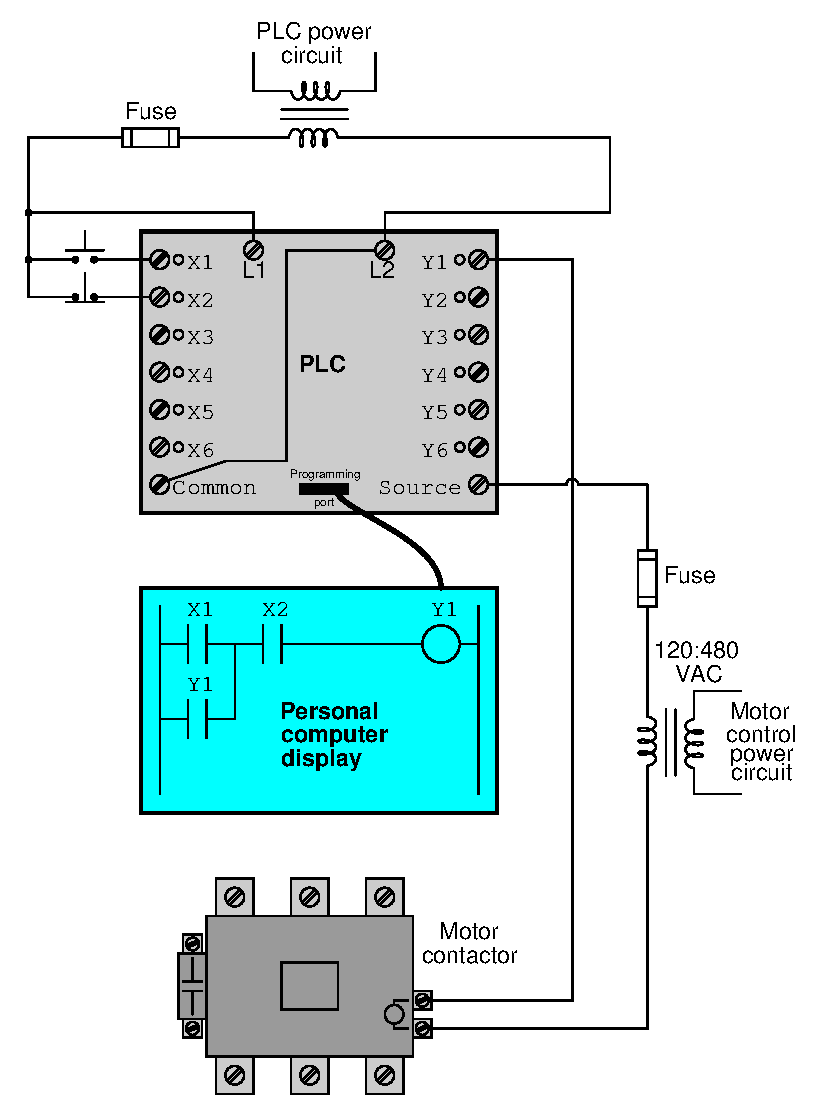
\includegraphics[width=15.5cm]{i02424x01.eps}$$

\filbreak

$$\includegraphics[width=15.5cm]{i02424x02.eps}$$

Under normal operating conditions, these two motor control systems will perform identically.  However, they will act differently under abnormal conditions.  Identify one such ``abnormal'' condition that will cause these two systems to act differently, and explain what that difference is.

\underbar{file i02424}
%(END_QUESTION)





%(BEGIN_ANSWER)

The latter system ``reads back'' the motor's status from the auxiliary contact on the contactor, rather than from a bit internal to the PLC (Y1).  This gives it the ability to ``sense'' what is going on in the real world.

\vskip 10pt

Imagine a case where the motor control power circuit fuse blew, preventing the motor contactor from energizing even when PLC output Y1 activates.  The internally-latched PLC program would blissfully maintain an energized condition on Y1 output after someone presses the Start pushbutton even though the motor is not running (and will suddenly start if anyone replaces the blown fuse!).  The externally-latched PLC program refuses to latch output Y1 on unless it senses the contactor has actually energized, making it a safer system.

\vskip 10pt

A similar system of external latching is used on electric clothes dryers, to latch the motor control circuit on only when an external speed switch senses drum rotation.  This prevents the unwanted condition of continuous motor and heater operation in the event of a broken belt (which would prevent the drum from turning).

%(END_ANSWER)





%(BEGIN_NOTES)




\vskip 20pt \vbox{\hrule \hbox{\strut \vrule{} {\bf Virtual Troubleshooting} \vrule} \hrule}

This question is a good candidate for a ``Virtual Troubleshooting'' exercise.  Presenting the diagram to students, you first imagine in your own mind a particular fault in the system.  Then, you present one or more symptoms of that fault (something noticeable by an operator or other user of the system).  Students then propose various diagnostic tests to perform on this system to identify the nature and location of the fault, as though they were technicians trying to troubleshoot the problem.  Your job is to tell them what the result(s) would be for each of the proposed diagnostic tests, documenting those results where all the students can see.

During and after the exercise, it is good to ask students follow-up questions such as:

\begin{itemize}
\item{} What does the result of the last diagnostic test tell you about the fault?
\item{} Suppose the results of the last diagnostic test were different.  What then would that result tell you about the fault?
\item{} Is the last diagnostic test the best one we could do?
\item{} What would be the ideal order of tests, to diagnose the problem in as few steps as possible?
\end{itemize}

%INDEX% PLC, ladder logic programming: external feedback in motor starter control

%(END_NOTES)


